\documentclass{prettytex/ox/mmsc-special-topic}
\usepackage{tabularray}
\usepackage{pdfpages}
\setlength{\headheight}{19.53pt}

\setcounter{biburllcpenalty}{7000}
\setcounter{biburlucpenalty}{8000}

\addbibresource{sources.bib}
\tikzexternalize[prefix=tikz/]

\newcommand{\topictitle}{
  Melon - a Task Scheduling Package for Todo List Applications \\
  \normalsize using Markov Chain Monte-Carlo Methods
}
\newcommand{\candidatenumber}{1072462}
\newcommand{\course}{Python in Scientific Computing}

\title{\topictitle}
\author{Candidate \candidatenumber}
\date{\today}

\makenoidxglossaries
\newacronym{mcmc}{MCMC}{Markov chain Monte-Carlo}
\newacronym{gui}{GUI}{Graphical User Interface}
\newacronym{caldav}{CalDAV}{Calendaring Extensions to WebDAV}
\newacronym{webdav}{WebDAV}{Web Distributed Authoring and Versioning}
\newacronym{ci}{CI}{Continuous Integration}
\newacronym{cd}{CD}{Continuous Delivery}
\newacronym{toml}{TOML}{Tom's Obvious, Minimal Language}

\begin{document}
  \pagestyle{plain}
  \mmscSpecialHeader

  \begin{abstract}
    \label{abstract}
    % In this project report we will review the central concepts utilised in the group work conducted to make progress in the \gls{pde} problem associated with the electrochemical model of a battery cell and present numerical results.
    \vspace*{0.2cm}

    % \noindent
    % \textbf{Our Goal:}
    % Numerically obtain the solution $\{a(x, T), b(x, T)\}$.

    The algorithm is implemented four times, twice in Python, once in Rust and also in C++.
    Python module bindings to these low-level language implementations are provided using \texttt{rust-cpython} and \texttt{pybind11}, respectively.
  \end{abstract}

  \begin{figure}[H]
    \centering
    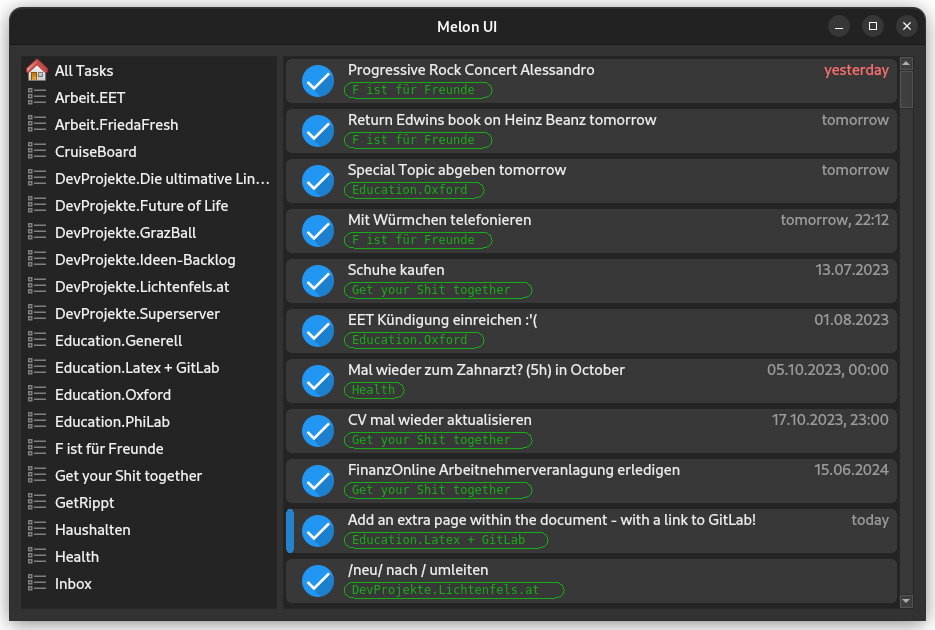
\includegraphics[width=0.85\linewidth]{figures/melon-ui.png}
    \caption{The \gls{gui} accompanying the scheduler. Double clicking tasks allows the user to edit them. Clicking the blue check icon marks them as completed. The grey text on the side represents the relevant due date. Selecting a calendar (todo-list) from the list on the left-hand side will filter the task list to only that category.}
    \label{fig:gui}
  \end{figure}

  \pagebreak
  \pagestyle{normal}

  % \tableofcontents

  \section{Problem Introduction}
  \label{sec:introduction}

  This report is concerned with finding a good scheduling approach for a given set of tasks (todos) with duration, priority, location and due date.
  The software attached with this report, going by the name of \textit{Melon}, consists of two parts: the \texttt{melon} task scheduling package itself and the Graphical User Interface written using the Qt6 framework, contained in \texttt{melongui}.
  Both of these are published as a package \textbf{melon-scheduler}, available \href{https://pypi.org/project/melon-scheduler/}{on PyPi}. It may be installed using

  \bashblock{pip install melon-scheduler}
  for just the scheduler, without the \gls{gui},

  \bashblock{pip install melon-scheduler[gui]} with the \gls{gui} or optionally,

  \bashblock{pip install melon-scheduler[gui,plots,numba]} with all extras.

  The package is capable of downloading and synchronising tasks from a calendar server supporting the industry-standard CalDAV protocol, displaying and editing them in the \gls{gui} and finally scheduling them into a calendar (cf. \Cref{fig:calendar}).
  The scheduling mechanism we implemented is a \gls{mcmc} method.

  \begin{figure}[H]
    \centering
    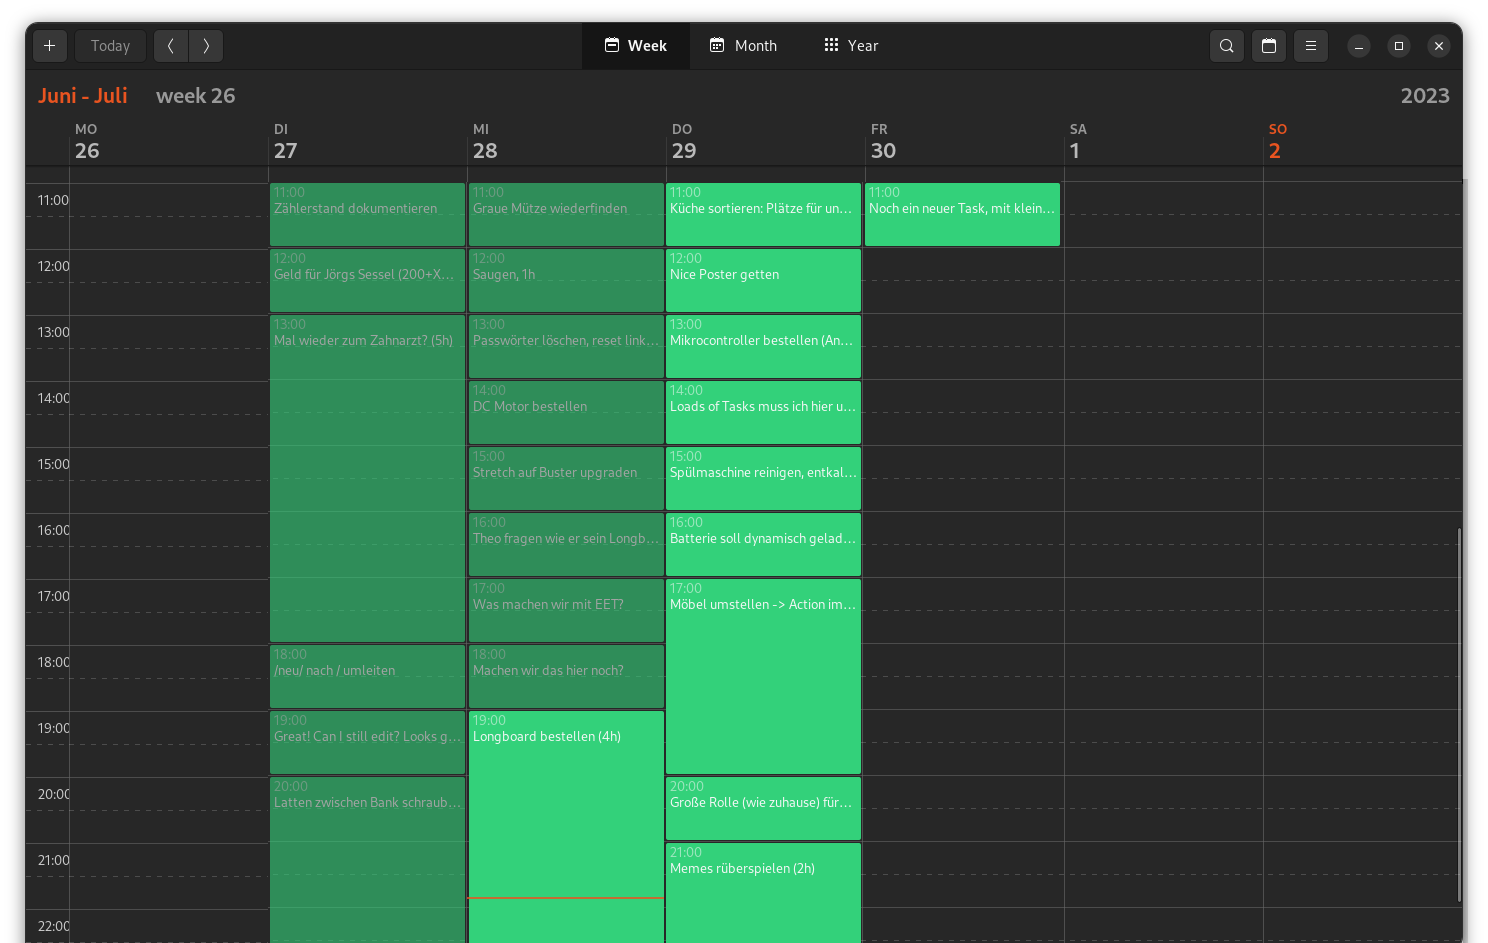
\includegraphics[width=\linewidth]{figures/exported-calendar.png}
    \caption{The scheduled tasks, as displayed in \textit{Gnome Calendar} (the default duration for each task is one hour). Theoretically existent events could be taken into account for task scheduling as well, just as well as breaks.}
    \label{fig:calendar}
  \end{figure}

  \subsection{Idea of the Algorithm}
  We work with the following assumption on the state: the entire scheduling, given the set of tasks, is solely determined by the order in which the tasks are scheduled.
  That is, for a given order of tasks, the full schedule can be created using the supplied input data.
  With this assumption, finding the absolute optimum is tedious, especially for a large number of tasks $N \gg 1$, as there are $N!$ possible ways to order the tasks.

  The idea of the Monte Carlo method implemented here is to minimise a penalty function (borrowing the term \textit{energy} from physics) over the discrete state space of size $\mathcal{O}(N!)$ using a stochastic approach, as sketched in \Cref{sec:theory}.
  The four key properties we aim to optimise for are:
  \begin{itemize}
    \tightlist
    \item spending a minimal amount of time to complete all tasks,
    \item scheduling high priority tasks first,
    \item a low number of commutes between locations and
    \item having all tasks completed on time.
  \end{itemize}
  Due to this choice of state representation, the problem broadly mimics a Traveling Salesman Problem.

  \section{Primer on the Underlying Theory}
  Many complex problems cannot be solved using analytical methods due to, for instance, their discrete nature.
  \gls{mcmc} methods with transition probabilities allow us to explore a huge state space regardless and minimise a function (energy $E$) therein.
  There are many use cases in physics, such as for the simulation of the Ising model, where the term \textit{energy} originates from.

  \label{sec:theory}
  \begin{algorithm}[language=pseudo,caption={\centering The Metropolis-Hastings sweep() sub-routine \parencite{metropolis, hastings}},basicstyle=\footnotesize]
for $N^2$ many times, repeat
  sample a candidate $\vec{x}^*$.
  set $\vec{x}^{n+1} = \vec{x}^*$ with acceptance probability
    $p_{\rm accept} = \min\left(1, \e^{-\beta (E^{n+1} - E^n)}\right)\,,$ with $\beta \in \R^+$ a transition factor.
  Otherwise, let $\vec{x}^{n+1} = \vec{x}^{n}$.
  \end{algorithm}

  Which is a subroutine to an outer iteration, a technique commonly referred to as Simulated Annealing.
  The idea of the iterative procedure above is to start from an initial state $\vec{x}^0$, permute it slightly and then accept that new proposal with a probability proportional to the exponential of their energy difference.
  If the proposal's energy is better (lower) than the current state's energy, the acceptance probability is $1$.
  This allows us to explore state space, but not get stuck in local minima as there is always a non-zero chance for the iteration to escape the local minimum.

  In our specific case, we will minimise the function $E(\vec{x})$ given in \Cref{eq:energy} based on the four properties stated above, using Metropolis-Hastings with Simulated Annealing.

  \begin{algorithm}[language=pseudo,caption={\centering Simulated Annealing},basicstyle=\footnotesize]
let k = 1
until convergence, repeat
  set the temperature $T = T_0 k^{q}$ and therefore $\beta = \frac{1}{T}$.
  perform a sweep()
  evaluate $\langle E\rangle$ and $\left\langle\Delta E^2\right\rangle$.
  set k = k + 1
  \end{algorithm}

  The key idea is to lower the temperature over the course of the simulation to reduce the transition probability.
  For each temperature $T$ we evaluate the average of the energy
  $$\langle E\rangle \simeq \frac{1}{n} \sum_{\vec{x}} E(\vec{x}), \quad \text { and } \quad\left\langle E^2\right\rangle \simeq \frac{1}{n} \sum_{\vec{x}} E^2(\vec{x})$$
  with $n$ the number of iterations for this temperature, hence the variance is given by
  $$\left\langle\Delta E^2\right\rangle:=\left\langle E^2\right\rangle-\langle E\rangle^2 \,.$$
  When the variance subceeds a certain threshold, one could stop the iteration.

  \section{Package Design and Architecture}
  The \glsname{caldav} format, short for the Calendaring Extensions to \gls{webdav} as introduced in \cite{caldav-rfc} defines three types of entities: VEVENTs, VTODOs and VJOURNALs.
  These entities are organised into calendars, for our purposes these could be thought of as different todo lists.
  \textit{Melon} interacts with CalDAV servers and objects through Python's \texttt{caldav} package.
  A decent amount of the code in \texttt{melon} and \texttt{melongui} is concerned with the interaction from the package to these objects.
  Within the scope of this report, we will focus on a smaller version of these VTODO objects, created for a swift interface to the scheduler algorithm implementations.

  This small object version, containing data relevant to the scheduling mechanism, looks like this:
  \begin{minted}{python}
    import dataclasses
    from datetime import datetime

    @dataclasses.dataclass
    class Task:
        uid: str  # unique identifier of the task
        duration: float  # estimated, in hours
        priority: int  # between 1 and 9
        location: int  # number indicating the location, 0 is "hybrid"
        due: datetime | None  # when the task is due
  \end{minted}

  So each task has an associated UID, duration, priority, location and due date.
  UIDs are useful because they make value collisions very unlikely.
  Which is not to say that these should not be checked, but if two separate calendar clients that each generated a set of UIDs, connected to a server, it is very unlikely to have to resolve potential conflicts.

  As mentioned above, the energy we minimise (to schedule the tasks) is a combination of four properties.
  To obtain our energy function, we propose numerical expressions for each of them (again, the lower, the better the state) and then perform a weighted sum over all four.
  Informally stated, the function we minimise is approximately given by
  \begin{align}
    \label{eq:energy} E(\vec{x}) = \; & \mathrm{slot~end}_N - \mathrm{slot~start}_1 + \sum_{j=1}^{N} \identity_{\mathrm{slot~end}_j > \mathrm{due}_j} \cdot 100                    \\
    \nonumber                         & + \sum_{j=2}^{n} (1 - \identity_{\mathrm{location}_{j-1}, \mathrm{location}_{j}}) \cdot 30 + \sum_{j=1}^{N} j \cdot \mathrm{priority}_j\,.
  \end{align}
  Results of the simulation may be found in \Cref{sec:results}.

  \subsection{Four Different Implementations}
  In order to compare runtimes, the same algorithm was implemented four times.
  Once in pure Python, once using the \texttt{numba} library and once in Rust and in C++.
  Numba uses Just-In-Time compilation to speed up subsequent calls of a subroutine.
  Rust and C++ are good choices for iterative procedures as they allow for low-level access to the implementation. Bindings are provided using \texttt{rust-cpython} and \texttt{pybind11}.

  \pagebreak
  \section{Installation and Usage}
  This project uses one of the latest versions of Python, 3.11.4.

  \subsection{Package Usage}
  After running \bash{pip install melon-scheduler[gui]} and starting a Python console, the following code snippet should start the \gls{gui}:

  \begin{minted}{python}
    from melongui.main import main
    main()  # to start the GUI
  \end{minted}

  which launches a User Interface such as the one depicted in \Cref{fig:gui}.

  To load todos from a remote calendar, as specified in the configuration file, and schedule them, use the following code-snippet:
  \begin{minted}{python}
    from melon.melon import Melon
    from melon.scheduler.rust import RustyMCMCScheduler

    melon = Melon()
    melon.autoInit()
    melon.scheduleAllAndExport("task-schedule.ics", Scheduler=RustyMCMCScheduler)
  \end{minted}

  In order to run the scheduler on demonstration data, please run
  \begin{minted}{python}
    from melon.scheduler.rust import RustyMCMCScheduler

    tasks = generateManyDemoTasks(N=80)
    scheduler = RustyMCMCScheduler(tasks)
    result = scheduler.schedule()
  \end{minted}

  If not specified in the initialiser, Melon loads a configuration file located in the user's home configuration directory, so on Linux \texttt{~/.config/melon/config.toml}.
  The file uses \gls{toml} format and has the following contents:
  \begin{minted}{toml}
[client]
url = "https://my-caldav-server.org:2023/dav/user/calendars/"
username = "user"
password = "password"
  \end{minted}

  \subsection{Full Project Usage}
  The ZIP file contains a number of configuration files at the top level, the two main code folders \texttt{melon} and \texttt{melongui}, \texttt{tests}, \texttt{docs} and the \texttt{report}.
  To install dependencies from the \texttt{pyproject.toml} file, please run

  \bashblock{poetry install}

  which will automatically create a virtual environment.

  There are two main entrypoints to running the code: \texttt{main.py} to run the GUI, as well as \texttt{tasks.py} which contains miscellanous development and analysis scripts. \textit{Melon} uses \texttt{invoke} to these common development tasks which are all callable by running

  \bashblock{inv (name-of-the-task) (arguments) (----keyword-arguments)}

  \begin{table}[H]
    \centering
    \caption{Running \bash{inv -l} yields a selection of available \texttt{invoke} tasks.}
    \begin{tblr}{colspec={X[5cm] X[\linewidth - 6cm]}}
      \texttt{build-docs}              & {Builds documentation using Sphinx.} \\
      \texttt{compare-runtime}         & {Compares runtime of the different scheduling implementations.} \\
      \texttt{compile}                 & {Assuming a full setup, compiles the low-level implementations of the scheduler algorithm in C++ and Rust.}\\
      \texttt{ipython-shell}           & {Starts an IPython shell with Melon initialised.} \\
      \texttt{plot-convergence}        & {Plots scheduler convergence to a file.} \\
      \texttt{plot-runtime-complexity} & {Simulates with a varying number of tasks and plots runtime complexity.} \\
      \texttt{profile-scheduler}       & {Profile the pure Python MCMC Scheduler.} \\
      \texttt{schedule-and-export}     & {Run the MCMC scheduler and export the resulting events as an ICS file.} \\
      \texttt{start-mock-server}       & {Starts a Xandikos (CalDAV) server on port 8000.}
    \end{tblr}
  \end{table}

  \paragraph{Low-Level Language Setup}
  In order to compile the C++ implementation of the scheduler algorithm, starting from the root folder of the project (containing \texttt{CMakeLists.txt} and \texttt{conanfile.txt}), please run

  \bashblock{conan install . ----output-folder=build ----build=missing} \\
  \bashblock{cd build} \\
  \bashblock{cmake .. -DCMAKE\_BUILD\_TYPE=Release} \\
  \bashblock{make -j4}

  To compile the Rust implementation, simply

  \bashblock{cargo build --release}

  again making sure that the current working directory is the root folder of the project (containing \texttt{Cargo.toml}).

  This should have created two \texttt{.so} files in the respective folders.
  The import paths are already adjusted to be able to import these in \texttt{cpp.py} and \texttt{rust.py}, but they will also be copied to the correct \texttt{melon/scheduler} folder using \bash{inv compile}.

  We recommend usage with \texttt{xandikos}, a version-controlled DAV server, capable of syncing calendars (events, todos and journals) and contacts.
  Following the standard protocol, \textit{Melon} is also compatible with commercial services such Google Calendar or Microsoft Office, as long as these offer an API endpoint with suitable authentication.

  The code should mostly be platform-independent, for example due to the usage of \texttt{pathlib.Path}. Compiling the low-level language implementations might be more cumbersome however and is untested on platforms other than Linux.

  \pagebreak
  \section{Code Quality Measures}
  Writing good code is an art, but there are a few concepts, principles and tools to approach the problem from a more standardised, scientific perspective.
  Some of these are:

  \paragraph{Formatting} the \textit{Melon} code is done by the \texttt{black} software package. Configuration thereof, as well as that for most other tools, can be found in the \texttt{pyproject.toml} file. To format all Python code, run \bash{black .} which will recursively explore the entire folder. The C++ code is formatted using \texttt{clang-format} while the Rust code is formatted using \texttt{rustfmt}.

  \paragraph{Docstrings} help us document the code, \textit{within} the code. Every class, method and function in the project, including \texttt{melon}, \texttt{melongui}, the \texttt{tasks} and the \texttt{tests}, has a docstring.
  This coverage can be verified using \bash{interrogate -vv}, cf. \Cref{table:interrogate}.

  \begin{table}
    \centering
    \caption{Result: \textcolor{green}{\bf Passed} (minimum: 80.0\%, actual: 100.0\%)}
    \begin{tabular}{lllll}
      \hline
      \bf Name                        & \bf Total & \bf Miss & \bf Cover & \bf Cover                 \\
      \hline
      main.py                         & 2         & 0        & 2         & \textcolor{green}{100 \%} \\
      tasks.py                        & 8         & 0        & 8         & \textcolor{green}{100 \%} \\
      docs/conf.py                    & 1         & 0        & 1         & \textcolor{green}{100 \%} \\
      melon/\_\_init\_\_.py           & 1         & 0        & 1         & \textcolor{green}{100 \%} \\
      melon/calendar.py               & 11        & 0        & 11        & \textcolor{green}{100 \%} \\
      melon/config.py                 & 1         & 0        & 1         & \textcolor{green}{100 \%} \\
      melon/melon.py                  & 19        & 0        & 19        & \textcolor{green}{100 \%} \\
      melon/todo.py                   & 20        & 0        & 20        & \textcolor{green}{100 \%} \\
      melon/visualise.py              & 3         & 0        & 3         & \textcolor{green}{100 \%} \\
      melon/scheduler/\_\_init\_\_.py & 1         & 0        & 1         & \textcolor{green}{100 \%} \\
      melon/scheduler/base.py         & 10        & 0        & 10        & \textcolor{green}{100 \%} \\
      melon/scheduler/cpp.py          & 3         & 0        & 3         & \textcolor{green}{100 \%} \\
      melon/scheduler/numba.py        & 8         & 0        & 8         & \textcolor{green}{100 \%} \\
      melon/scheduler/purepython.py   & 12        & 0        & 12        & \textcolor{green}{100 \%} \\
      melon/scheduler/rust.py         & 3         & 0        & 3         & \textcolor{green}{100 \%} \\
      melongui/\_\_init\_\_.py        & 1         & 0        & 1         & \textcolor{green}{100 \%} \\
      melongui/calendarlist.py        & 6         & 0        & 6         & \textcolor{green}{100 \%} \\
      melongui/mainwindow.py          & 14        & 0        & 14        & \textcolor{green}{100 \%} \\
      melongui/taskitemdelegate.py    & 12        & 0        & 12        & \textcolor{green}{100 \%} \\
      melongui/tasklist.py            & 14        & 0        & 14        & \textcolor{green}{100 \%} \\
      melongui/taskwidgets.py         & 8         & 0        & 8         & \textcolor{green}{100 \%} \\
      tests/\_\_init\_\_.py           & 1         & 0        & 1         & \textcolor{green}{100 \%} \\
      tests/test\_melon.py            & 7         & 0        & 7         & \textcolor{green}{100 \%} \\
      tests/test\_scheduler.py        & 9         & 0        & 9         & \textcolor{green}{100 \%} \\
      \hline
      \bf TOTAL                       & 175       & 0        & 175       & \textcolor{green}{100 \%} \\
      \hline
    \end{tabular}
    \label{table:interrogate}
  \end{table}

  \paragraph{Documentation} is important to make the purpose and usage of the code package clear. This project uses \texttt{sphinx} to generate documentation in PDF format which one may find at the end of this report. To generate the documentation, run \bash{inv build-docs}.

  \paragraph{Dependency Management} in this project is done using \texttt{poetry}, which not only manages install packages and manages virtual environments, but also keeps track of dependency groups.
  To install all direct dependencies, run \bash{poetry install}.

  \paragraph{Type Checking} is done with \texttt{pyright} instead of \texttt{mypy} as it is much faster and analyses the entire project at once. This tool detects when, for instance, attempting to call a non-existent method on an object, or passing the wrong type to a function call, etc.
  The \textit{Melon} code therefore contains numerous type hints.
  To verify all type hints, run \bash{pyright .} in the root folder of the project.

  \paragraph{Using Appropriate Language Features}
  Tools such as \texttt{autoflake} and \texttt{pyupgrade} automatically correct unused imports or deprecated code usage.
  \texttt{ruff} is a highly performant linter written in Rust, that not only warns the programmer on common mistakes, but can also perform small fixes to the structure of the code such as import reordering.
  \texttt{nitpick} is a tool to synchronise linter configuration across projects.

  \subsection{Tests and Coverage}
  Software testing is a vital part of any programming endeavour to ensure high levels of overally code quality.
  This submission only contains tests for the \texttt{melon} package of the code, not for the \gls{gui}, which will be subject to future efforts.
  There are 34 tests provided along with the code.

  In order to simulate the interaction with a \gls{caldav} server, we provide a tool to start a mock server using Docker, a containerisation engine that abstracts code execution to individual entities called containers.
  To start a the \texttt{xandikos} mock server, please run

  \bashblock{inv start-mock-server}

  Once the server is running, the tests may be run simply by:

  \bashblock{pytest}

  As we can see using \bash{pytest ----durations=0},

  \texttt{
    ========================= slowest durations ========================= \\
    3.53s call TestScheduler::test\_length[NumbaMCMCScheduler] \\
    0.19s call TestMelon::test\_init\_store\_and\_load
  }

  the slowest test is the first routine involving the Numba scheduler which takes some time to pre-compile the functions.
  So even when the runtime of the Numba scheduler itself is low (cf. \Cref{sec:runtime}), the test will always take some extra time.

  \subsubsection{Code Coverage}
  \begin{table}[H]
    \centering
    \caption{Test coverage of the \texttt{melon} package: platform linux, python 3.11.4-final-0. This table may be reproduced using \bash{pytest ----cov=melon}.}
    \begin{tabular}{lrrr}
      \hline
      \bf Name                        & \bf Statements & \bf Miss & \bf Cover                    \\
      \hline
      melon/\_\_init\_\_.py           & 0              & 0        & \textcolor{green}{100 \%}    \\
      melon/calendar.py               & 57             & 5        & \textcolor{green}{91 \%}     \\
      melon/config.py                 & 12             & 0        & \textcolor{green}{100 \%}    \\
      melon/melon.py                  & 121            & 8        & \textcolor{green}{93 \%}     \\
      melon/scheduler/\_\_init\_\_.py & 0              & 0        & \textcolor{green}{100 \%}    \\
      melon/scheduler/base.py         & 40             & 3        & \textcolor{green}{92 \%}     \\
      melon/scheduler/cpp.py          & 18             & 5        & \textcolor{green}{72 \%}     \\
      melon/scheduler/purepython.py   & 83             & 0        & \textcolor{green}{100 \%}    \\
      melon/scheduler/rust.py         & 18             & 5        & \textcolor{green}{72 \%}     \\
      melon/todo.py                   & 101            & 17       & \textcolor{green}{83 \%}     \\
      melon/visualise.py              & 42             & 2        & \textcolor{green}{95 \%}     \\
      \hline
      \bf TOTAL                       & \bf 492        & \bf 45   & \bf \textcolor{green}{91 \%}
    \end{tabular}
  \end{table}

  \paragraph{Maintaining Code Quality}
  \texttt{pre-commit} is a tool that can install a git hook to the code repository, which automatically runs a set of checks before every commit, hence the name.
  For this project, various checks listed below are employed, being run before each and every commit to keep code quality high throughout the entire development process.

  \texttt{
    \hspace*{-1em} prettier........................................................\textcolor{green}{Passed} \\
    fix end of files................................................\textcolor{green}{Passed} \\
    trim trailing whitespace........................................\textcolor{green}{Passed} \\
    black...........................................................\textcolor{green}{Passed} \\
    ruff............................................................\textcolor{green}{Passed} \\
    check blanket noqa..............................................\textcolor{green}{Passed} \\
    check for eval()................................................\textcolor{green}{Passed} \\
    interrogate.....................................................\textcolor{green}{Passed} \\
    autoflake.......................................................\textcolor{green}{Passed} \\
    pyupgrade.......................................................\textcolor{green}{Passed} \\
    pyright.........................................................\textcolor{green}{Passed} \\
    pytest-check....................................................\textcolor{green}{Passed} \\
    clang-format....................................................\textcolor{green}{Passed} \\
    latex-format-all................................................\textcolor{green}{Passed}
  }

  A similar, more team-friendly option is to use GitHub Actions \gls{ci} / \gls{cd}, or simply CI/CD.

  \paragraph{Publishing to PyPi}
  As highlighted above, the project can be installed from \href{https://pypi.org/project/melon-scheduler/}{this PyPi repository}.
  In order to build and publish the project, one can simply run

  \bashblock{poetry publish --build}

  Although it would be possible to compile the C++ and Rust implementations on a CI service using a ``platform matrix'', the published package only contains compilation targets for the x86\_64 platform and Python 3.11.

  All the tools described above will be installed automatically using \bash{poetry install --with=dev}.

  \section{Results}
  \label{sec:results}
  \subsection{Algorithm Convergence}
  \label{sec:convergence}
  \begin{figure}[H]
    \centering
    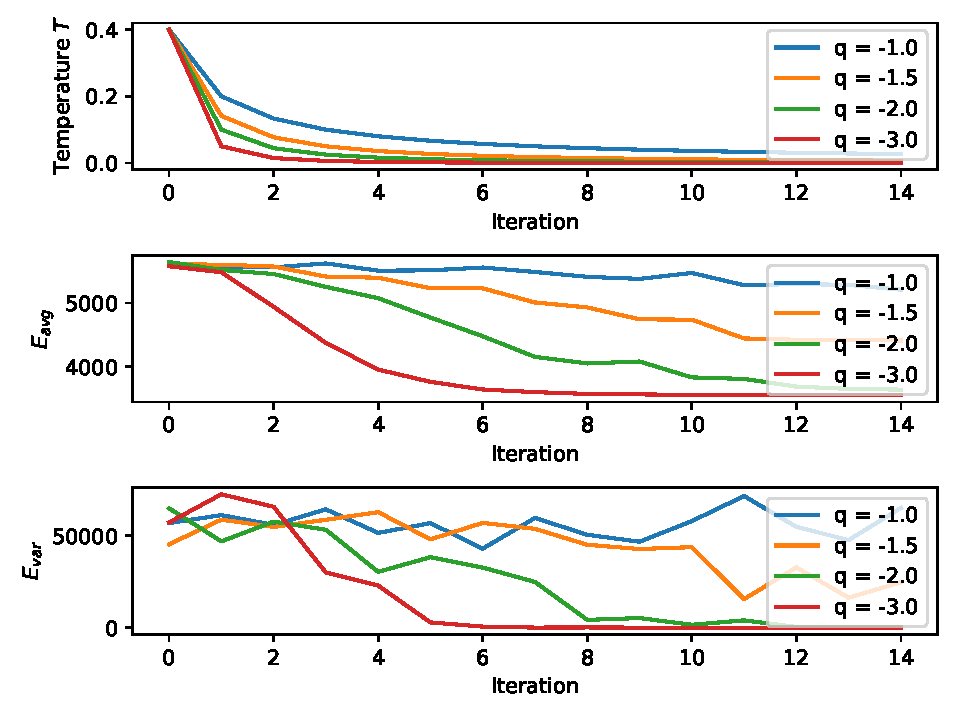
\includegraphics[width=0.8\linewidth]{results/convergence-8h-day.pdf}
    \caption{Temperature, average energy and energy variance for an 8-hour work day. Low variance can be used as a stopping criterion (cf. \Cref{sec:theory}).}
  \end{figure}
  \begin{figure}[H]
    \centering
    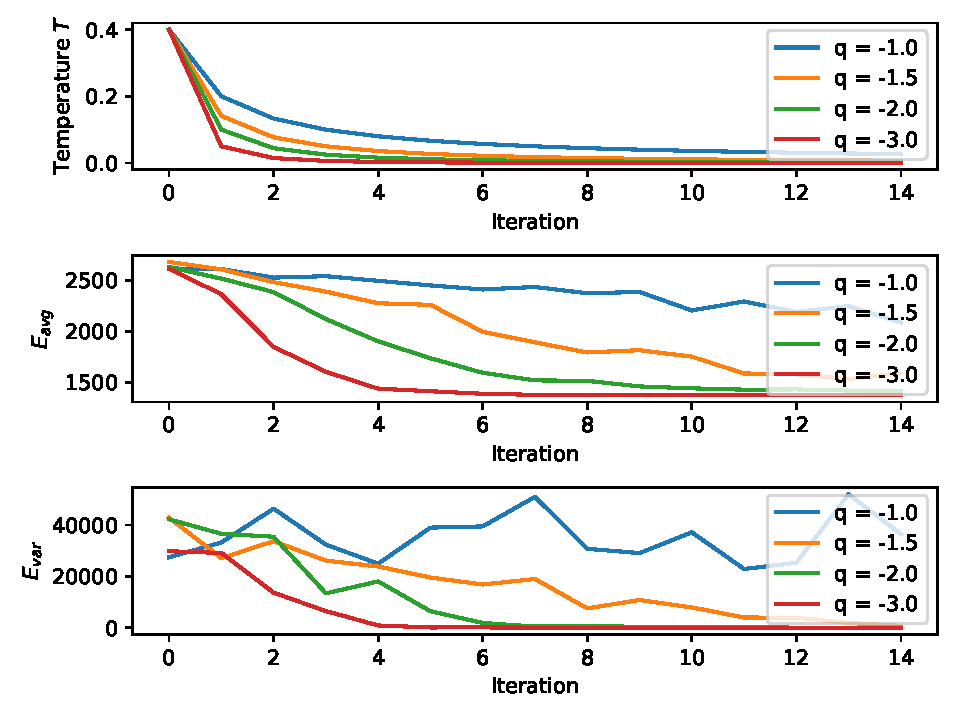
\includegraphics[width=0.8\linewidth]{results/convergence-14h-day.pdf}
    \caption{Temperature, average energy and energy variance for a 14-hour work day.}
  \end{figure}

  \subsection{Runtime Performance}
  \label{sec:runtime}
  The following benchmarks were all accumulated on an x86\_64 Intel\textregistered \, i7-5600U CPU running at \SI{2.6}{\giga\hertz} verified through 3 individual runs, keeping parameters consistent along them.

  \begin{figure}[H]
    \centering
    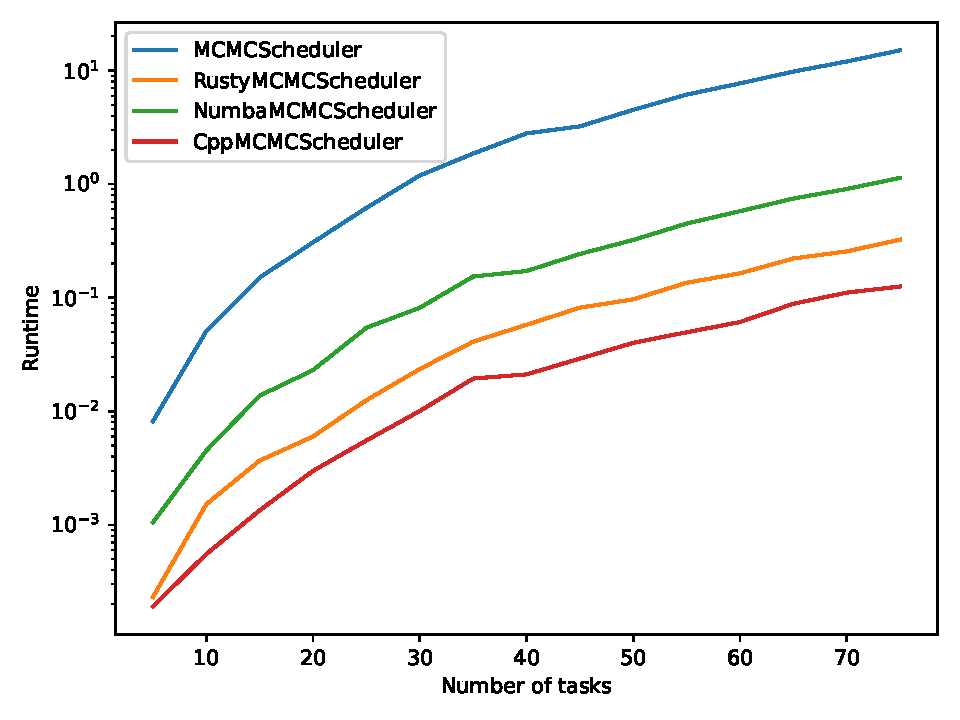
\includegraphics[width=0.7\linewidth]{results/complexity.pdf}
    \caption{Complexity plot}
  \end{figure}

  \begin{table}[H]
    \vspace{0.5cm}
    \centering
    \caption{Runtime Comparison of the different implementations run on the same scenarios. Each runtime is given as the average over three runs.}
    \begin{tblr}{
      colspec={llr},
      row{2,3} = {bg=azure9},
          row{4} = {bg=violet9},
          row{5} = {bg=cyan9},
        }
      \hline
      \bf Implementation & \bf Language & \bf Runtime / seconds \\
      \hline
      MCMCScheduler      & Python & 31.3887 \\
      NumbaMCMCScheduler & Python & 1.9335 \\
      \hline
      RustyMCMCScheduler & Rust & 0.4034 \\
      \hline
      CppMCMCScheduler   & C++ & 0.4062
      \hline
    \end{tblr}
    \label{table:runtime}
  \end{table}

  Regarding the table above, one should note that the Numba compilation time was approximately 3.2 seconds, which takes place once for each Python process.

  \begin{table}[H]
    \centering
    \caption{Profile obtained by running \mintinline{bash}{inv profile-scheduler | grep purepython.py}.}
    \begin{tabular}{rrrrrll}
      \hline
      \bf Ncalls & \bf Total & \bf / call & \bf Cum. & \bf / call & \bf Filename:line & \bf Function     \\
      \hline
      1          & 0.000     & 0.000      & 14.236   & 14.236     & purepython:142    & schedule         \\
      10         & 0.209     & 0.021      & 14.235   & 1.424      & purepython:123    & mcmcSweep        \\
      36010      & 1.144     & 0.000      & 13.784   & 0.000      & purepython:97     & computeEnergy    \\
      2196671    & 5.391     & 0.000      & 11.353   & 0.000      & purepython:41     & spreadTasks      \\
      1006332    & 1.389     & 0.000      & 1.842    & 0.000      & purepython:27     & generateNextSlot \\
      2196610    & 0.798     & 0.000      & 0.972    & 0.000      & purepython:108    & <genexpr>        \\
      2196610    & 0.384     & 0.000      & 0.384    & 0.000      & purepython:106    & <genexpr>        \\
      36000      & 0.082     & 0.000      & 0.217    & 0.000      & purepython:83     & permuteState     \\
      36011      & 0.046     & 0.000      & 0.124    & 0.000      & purepython:19     & startingSlot     \\
    \end{tabular}
  \end{table}

  \section{Acknowledgements}
  The visualisation code (\texttt{visualise.py}) is adapted from \cite{monte-carlo-todo-lists}.

  The task check icon is the logo of the \textit{Tasks.org} Free and Open Source Android App, which may be found \href{https://github.com/tasks/tasks/tree/main/graphics}{here}.

  \pagebreak
  \printbibliography
  \printnoidxglossary[type=acronym]

  \appendix
  \section{Accessing VTODO properties}
  A profiler may be used to identify parts of the code that are slow.
  In the case of the \gls{gui}, the Item Delegate's paint() method must be performant in order to provide a smooth user experience.
  This can be achieved when looking at different means of accessing the UID of a task, which as per \Cref{table:paint-profile} is a highly frequent action.
  Here is a comparison of different approaches:

  \begin{minted}{python}
    In [1]: %timeit str(t.icalendar_component["uid"])
      122 µs ± 1.06 µs per loop (7 runs, 10,000 loops each)
    In [2]: %timeit t.vtodo.contents["uid"][0].value
      355 ns ± 7.14 ns per loop (7 runs, 1,000,000 loops each)
    In [3]: %timeit t.vobject_instance.contents["vtodo"][0].contents["uid"][0].value
      296 ns ± 7.06 ns per loop (7 runs, 1,000,000 loops each)
    In [4]: %timeit t._vobject_instance.contents["vtodo"][0].contents["uid"][0].value
      208 ns ± 23.7 ns per loop (7 runs, 10,000,000 loops each)
  \end{minted}

  As we can see, the last option is the fastest which has therefore been implemented in \texttt{todo.py}.

  \begin{table}[H]
    \centering
    \caption{Profile obtained by running \mintinline{bash}{./main.py --profile | grep todo.py}.}
    \begin{tabular}{rrrrrll}
      \hline
      ncalls & tottime & percall & cumtime & percall & filename:lineno & function     \\
      \hline
      16958  & 0.008   & 0.000   & 0.939   & 0.000   & todo.py:36      & vtodo        \\
      32475  & 0.047   & 0.000   & 0.705   & 0.000   & todo.py:96      & uid          \\
      856    & 0.003   & 0.000   & 0.579   & 0.001   & todo.py:26      & upgrade      \\
      117    & 0.000   & 0.000   & 0.489   & 0.004   & todo.py:111     & priority     \\
      417    & 0.001   & 0.000   & 0.461   & 0.001   & todo.py:121     & isIncomplete \\
      5512   & 0.003   & 0.000   & 0.278   & 0.000   & todo.py:45      & summary      \\
      856    & 0.002   & 0.000   & 0.112   & 0.000   & todo.py:21      & \_\_init\_\_ \\
      1363   & 0.006   & 0.000   & 0.024   & 0.000   & todo.py:164     & \_\_lt\_\_   \\
      7844   & 0.004   & 0.000   & 0.009   & 0.000   & todo.py:61      & dueDate      \\
      2605   & 0.001   & 0.000   & 0.003   & 0.000   & todo.py:85      & dueTime      \\
    \end{tabular}
    \label{table:paint-profile}
  \end{table}

  \includepdf[pages=7-29]{../build/docs/latex/melon.pdf}
\end{document}
